\section{Differential expression and splicing analyses}

This section describes the statistical expression and splicing analyses that were performed following the pre-processing and filtering of our long-read sequencing data in \textbf{Chapters 5 and 6}. The aim was to identify statistically significant differences in expression, splicing and usage of genes and transcripts between experimental groups. Parameters that are specific to individual results chapters can be found in the Method section of the relevant chapter. 

\subsection{Gene and isoform quantification}\label{sec: gene_isoform_quant_explained}
Any differential expression analysis first requires an estimation of the gene and/or transcript expression. In handling the short-read nature of RNA-Seq data, previous bioinformatic tools and computational models have determined this primarily from the number of reads that align to each transcript sequence from a reference genome annotation\cite{Conesa2016} (\cref{fig:isoform_quant_strategy}\textbf{A}). While such approaches can accurately determine gene expression, it becomes much more challenging to estimate transcript expression due to the overlapping exonic structure of related transcripts, resulting in ambiguous read assignment (previously illustrated in \cref{fig:rna_seq_limitations}). Several sophisticated algorithms have been developed, including the Expectation-Maximization (EM) algorithm (adopted in \textit{Kallisto}\cite{Bray2016} and \textit{RSEM}\cite{Li2011}), which assign reads to multiple genomic loci and work without a reference genome\cite{Conesa2016}. 

The advent of long-read transcript sequencing data and the availability of matched short-read RNA-Seq data enabled gene and isoform expression to be estimated in two ways: i) a hybrid approach that involves mapping RNA-Seq data to Iso-Seq-derived or ONT-derived transcripts (\cref{fig:isoform_quant_strategy}\textbf{B}), or ii) directly using the normalised full-length read count from long reads as a proxy of gene and transcript expression (\cref{fig:isoform_quant_strategy}\textbf{C}); notably, the gene expression is estimated from the summation of full-length read counts from associated transcripts. While the former hybrid approach still suffers from ambiguous alignment to a degree, usage of the long-read-defined transcriptome in place of the reference genome would minimise misalignment, and improve mapping to condition-specific transcripts and other novel transcripts that are otherwise missing in the reference annotations\cite{Au2013}. Conversely, the latter approach does not rely on transcript assembly and is thus not impeded by misalignment. However, long-read sequencing data from global transcriptome profiling is still often considered semi-quantitative in most instances, due to the insufficient coverage required to detect expression changes.

\begin{figure}[htp]
	\begin{center}
		\includegraphics[page=8,trim={2cm 19cm 2cm 1cm},clip, scale = 0.8]{Figures/ProjectDevelopment_Figures.pdf}
	\end{center}
	\captionsetup{width=0.95\textwidth}
	\caption[Strategies for isoform quantification]%
	{\textbf{Strategies for isoform quantification.} Shown is a schematic diagram of the three strategies adopted for determining isoform abundance: \textbf{(A)} RNA-Seq reads (blue lines) aligned to the reference genome (black boxes, approach adopted in previous transcriptome profiling studies), \textbf{(B)} a hybrid approach that involves aligning RNA-Seq reads (blue lines) to the long-read-defined transcriptome (orange boxes), or \textbf{(C)} directly using normalised full-length read counts from long reads. Long reads refer to both Iso-Seq and ONT reads.}
	\label{fig:isoform_quant_strategy}
\end{figure}


\subsection{Differential gene and transcript expression analyses}
Differential gene expression (DGE\nomenclature{DGE}{Differential gene expression}) or transcript expression analysis (DTE\nomenclature{DTE}{Differential transcript expression}) identifies genes or transcripts that have a statistically significant change in abundance across biological conditions (i.e. identifying features that are “differentially expressed”) (\cref{fig:dte_dtu_explanation}\textbf{A}). To facilitate unbiased comparisons across samples and experimental groups, raw read counts are normalised to eliminate feature-length and library-size effects - longer transcripts and samples sequenced at a higher depth would accumulate more reads - to a standard metric, namely TPM (Transcripts per million\nomenclature{TPM}{Transcripts per million}). Full-length reads from long-read sequencing are thus normalised to TPM using the following equation: 

\begin{myequation}[!h]
	\begin{equation}
		FL\;\:TPM (x_{sample},y_{sample})=\frac{Raw\;\:FL\;\:count (x_{isoform},y_{sample})}{Total\;\:FL\;\:count (y_{sample})} *10^6
	\end{equation}
\end{myequation}
%With a cut-off lower than 0.5 TPM, a 0.5 - 10 TPM refers to low expression, a 11- 1000 refers to medium expression, and > 1000 TPM high expression [literature ref]. 

Between-sample normalisation methods, such as TMM\cite{Robinson2010} (Trimmed mean of M-values\nomenclature{TMM}{Trimmed mean of M-values}), are also used to account for differences in sample RNA library composition. This is particularly important when comparing samples between differential experimental groups with varying library composition. 

While significant computational advances have been made in processing long-read data for transcriptome annotations, methods to harness such data for downstream differential expression analyses have been limited. Current differential expression analyses of long-read sequencing data typically rely on existing tools originally developed for short-read RNA-Seq\cite{Amarasinghe2020}, such as \textit{DESeq}, \textit{maSigPro}, \textit{edgeR}, among others. Highlighting the challenges of performing such analyses, various benchmarking studies have demonstrated that the choice of tool can affect the outcome considerably and no single method performs favourably across all datasets. Notably, tools based on negative binomial modelling performed better with higher specificity and sensitivity\cite{Rapaport2013}. Recent methods, such as \textit{FLAIR} and \textit{LIQA}\cite{Hu2021}, have emerged specifically for isoform expression analysis of long-read data. However, such methods have not been systematically assessed and are challenging to use for time-series data analyses; our targeted experiments in \textbf{Chapters 5 and 6} include data from two different conditions and across four time points. 

\subsection{Differential splicing analysis}\label{intro:dtu}
A change in alternative splicing can be assessed in two ways: i) differential transcript expression (DTE), as described above, defined by a change in \textit{absolute} expression of a transcript, and ii) differential transcript (or isoform) usage (DTU\nomenclature{DTU}{Differential transcript usage}) defined by a change in the \textit{relative} expression of a transcript, manifesting to a change in the proportions of the transcript (or isoform) of a gene (\cref{fig:dte_dtu_explanation}\textbf{B}). As shown in \cref{fig:dte_dtu_explanation}, DTU always implies DTE whereas the reverse is not necessarily true; e.g. a two-fold increase of two associated isoforms results in a change in the absolute but not the relative expression (\cref{fig:dte_dtu_explanation}\textbf{A}), indicating a transcription-related mechanism. Conversely, any change in relative abundance of isoforms indicate a splicing-related mechanism. We observed examples of these mechanisms, notably in \textit{Trem2} (later described in \cref{trem2_diff}) and \textit{Bin1} (later described in \cref{bin1_diff}) from targeted profiling of the rTg4510 cortex.

One phenomenon characterised in differential splicing analysis is the significant altering of isoform proportions (also known as “Isoform Fraction”), resulting in the detection of a different dominant isoform. This phenomenon is known as “major isoform switching” (\cref{fig:dte_dtu_explanation}\textbf{C}). In this circumstance, the same isoform is predominantly expressed in one condition (where it is the major isoform), but is lowly expressed in another (where it is the minor isoform). Notably, up-regulation of one isoform could be compensated by down-regulation of another, resulting in no net change at the gene-level (\cref{fig:dte_dtu_explanation}\textbf{D}). Transcriptomic profiling studies at the gene-level would thus fail to capture such nuances, highlighting the complexity of gene regulation and the importance of performing differential expression analysis at a transcript-level. 


\begin{figure}[htp]
	\begin{center}
		\includegraphics[page=20,trim={0cm 12cm 0 0cm},clip, scale = 0.8]{Figures/ProjectDevelopment_Figures.pdf}
	\end{center}
	\captionsetup{width=0.95\textwidth,singlelinecheck=off}
	\caption[Scenarios of differential splicing]%
	{\textbf{Scenarios of differential splicing.} Shown is a schematic illustration of four different scenarios envisioned under differential splicing of a gene with two isoforms between conditions 1 and 2:
	\begin{enumerate}[label=\textbf{\Alph*})]
		\item Differential transcript expression (DTE) indicates an expression change for at least one transcript between conditions 1 and 2. However, the expression proportion of each transcript (defined as percentage of the total expression of all associated transcripts, in this case 50\% for Isoform B) remains constant.
		\item Conversely in differential transcript usage (DTU), the relative expression of the isoforms is changed across conditions - in this case, Isoform B has a relative expression of 33.3\% in condition 1 (5/15), but a relative expression of 41.6\% in condition 2 (10/24).
		\item Differential transcript usage can occur with a switch of the major isoform - in this case, the more abundantly expressed isoform is switched from Isoform A in condition 1 to Isoform B in condition 2. 
		\item Differential transcript usage can result in no overall change in gene expression if the change of transcript expression occurs in opposite directions.
		\\
	\end{enumerate} 
	Figures and legends were adapted from Soneson et al. (2016)\cite{Soneson2016}. 
   }
	\label{fig:dte_dtu_explanation}
\end{figure}

Despite the limited utility of short-read RNA-Seq data for elucidating differential splicing events, a number of computational methods have been developed (reviewed in \cref{tab: rnaseq_diffsplicing}), and are based around two major strategies: i) isoform-based and ii) count-based methods, which are further subdivided into exon-based and event-based. Isoform-based methods aim to reconstruct the transcripts from sequencing reads and estimate the relative abundance in each sample, followed by statistical testing to identify transcripts with significant expression differences across experimental groups\cite{Mehmood2020}. Conversely count-based methods dissect genes into counting units and document the number of reads falling within those units\cite{Mehmood2020}; exon-based methods assign reads into exonic and junction regions, whereas event-based methods quantify transcripts by measuring the inclusion of individual splicing events with a percent splicing index (PSI\nomenclature{PSI}{Percent splicing index}) value for each event (i.e. proportion of associated isoforms that contain the splicing event of interest). 

However, similar to transcript quantification, there is no clear consensus about the optimal tool or pipeline for such analysis. Benchmarking studies have similarly revealed that the choice of tools can directly impact the sensitivity and precision to detect differential transcripts, which are influenced by the number of replicates and the conditions heterogeneity\cite{Merino2019}. Exon-based methods (i.e. \textit{DEXSeq, edgeR, limma}) were found to overall perform better (superior precision and sensitivity) than other methods, with \textit{edgeR} recommended for faster performance and reduced memory requirements\cite{Mehmood2020}. 


\newgeometry{left=2.7cm,bottom=1.5cm, right=1.5cm, top=1.5cm}
\begin{landscape}
	\small %smaller font
	\setlength\tabcolsep{2pt} %reduced margin size in table
	\renewcommand{\arraystretch}{1}
\begin{longtable}[c]{p{2.5cm}p{2cm}p{2cm}p{1.5cm}p{17.5cm}}
	\caption[Bioinformatic approaches and tools to perform differential splicing analysis]%		
	{\textbf{Bioinformatic approaches and tools to perform differential splicing analysis.} Tabulated is an overview of some of the more commonly used bioinformatic approaches and tools for differential splicing analysis. \newline AS - Alternative splicing, AF - Alternative first exon, IR - Intron retention, MX - Mutually exclusive, ES - Exon skipiping. Table is adapted from Mehmood et al. (2020)\cite{Mehmood2020} and is by no means comprehensive. }
	\label{tab: rnaseq_diffsplicing}\\
	\toprule
	Approach &
	Method &
	Annotation &
	Designs &
	Model \\ \midrule
	\multirow{2}{*}{Isoform-based} &
	\textit{Cufflinks} \newline /\textit{cuffdiff2} &
	Yes, \textit{de novo} &
	2 groups &
	\tabitem Following transcript assembly, transcript abundance is estimated by maximising the likelihood score across all possible combinations of relative abundances of each associated isoform. \newline 
	\tabitem Variability between replicates and uncertainty in abundance are accounted with a beta negative binomial model. \\ 
	
	&
	\textit{DiffSplice} &
	\textit{Ab initio} &
	2 groups &
	\tabitem Reconstructs a graph of the transcriptome based on reads, from which the abundance is estimated from alternative paths and alternative splicing modules.\newline 
	\tabitem  Abundance of modules is compared using a non-parametric permutation test. \\ \cmidrule(l){1-5} 
	\multirow{4}{*}{Exon-based} &
	\textit{DEXSeq} &
	Yes &
	Complex &
	\tabitem Applies a generalised linear model to exon-level expression data to model differential usage of exons across experimental groups, assuming that read counts follow a negative binomial distribution. \\ 		
	&
	\textit{edgeR} &
	Yes &
	Complex &
	\tabitem Fits a negative binomial generalised log-linear model to exon-level expression data to test differential exon usage by comparing the log-fold-change of an exon to that of the gene. \\
	&
	\textit{JunctionSeq} &
	Yes, \textit{de novo} &
	Complex &
	\tabitem Uses a similar statistical method as \textit{DEXSeq} with added features to include novel exon junctions in differential exon usage analysis. \\	
	&
	limma &
	Yes &
	Complex &
	\tabitem Fits a linear model to exon-level expression data for differential exon usage between experimental groups \\ \cmidrule(l){1-5} 
	\multirow{4}{*}{Event-based} &
	\textit{dSpliceType} &
	Yes &
	2 groups &
	\tabitem For each AS event type (ES, RI, MX, A3SS, A5SS), it calculates the read coverage signal for each base and the normalised logarithmic ratios of PSI between groups. Differential splicing events are then identified using a parametric test on the PSI. \\ 			
	& 
	\textit{MAJIQ} &
	Yes, \textit{de novo} &
	2 groups &
	\tabitem Uses local splicing variations, which denote splits in a splice graph mapping to the edges of a reference exon to calculate PSI.   
	\tabitem Changes in PSI are then quantified using Bayesian modelling and bootstrapping. \\ 		

	&
	\textit{rMATS} &
	Yes &
	2 groups, \newline paired samples &
	\tabitem Calculates PSI for each AS event after applying a hierarchical framework to account for within-sample uncertainty and between-sample variability.
	\tabitem Mean PSI across each AS event is then tested between experimental conditions using a likelihood ratio. \\ 	
	&
	\textit{SUPPA2} &
	Yes &
	2 groups, \newline paired samples &
	\tabitem Determines transcript abundance using RSEM to estimate PSI   for each AS event \\* \bottomrule 
	\end{longtable}
\end{landscape}
\restoregeometry

\subsection{TappAS: Integrated framework for differential expression and splicing analyses}\label{ch3_tappas_explained}
After trialling various methods, we selected \textit{tappAS}\cite{DeLaFuente2020} (v1.0.0) as a framework for the differential expression and splicing analyses of long-read sequencing data across biological conditions (i.e. AD vs non-AD) in this thesis (\textbf{Chapters 5 and 6}). To date, it is the only tool that allows integration of isoform-level, long-read-derived annotations with public databases to comprehensively understand the functional implications of alternative splicing. Accessible as a user-friendly Java application, it provides the flexibility to incorporate expression derived from short-reads or long-reads, and supports complex design experiments: i) case-control, ii) time-course single series, and iii) time-course multiple series. Developed by the same authors as \textit{SQANTI}\cite{Tardaguila2018}, it was recommended as an extension to the Iso-Seq bioinformatics pipeline for downstream isoform-level analyses.    

The following sections detail specific analyses from \textit{tappAS} in investigating differential expression and splicing changes associated with progressive tau pathology in rTg4510 mice at a global (\textbf{Chapter 5}) and targeted level (\textbf{Chapter 6}). All details are summarised from Lorena de la Fuente et al. (2020)\cite{DeLaFuente2020}.

\vspace{2cm}
\begingroup
\parindent=0em
\etocsettocstyle{\rule{\linewidth}{\tocrulewidth}\vskip0.5\baselineskip}{\rule{\linewidth}{\tocrulewidth}}
\etocsetnexttocdepth{5}
\localtableofcontents 
\endgroup


\begin{figure}[htp]
	\begin{center}
		\includegraphics[page=21,trim={0cm 5cm 0 0cm},clip, scale = 0.8]{Figures/ProjectDevelopment_Figures.pdf}
	\end{center}
	\captionsetup{width=0.95\textwidth,singlelinecheck=off}
	\caption[Differential expression and splicing analyses of long-reads using \textit{tappAS}]%
	{\textbf{Differential expression and splicing analyses of long-reads using \textit{tappAS.}} Shown is \textbf{(A)} the \textit{tappAS} project creation workflow, which requires three input files: a transcript-level expression matrix, an experimental design file and a transcript-level functional annotation file. The expression matrix can be obtained from mapping RNA-Seq data to a long-read-defined transcriptome (\cref{fig:isoform_quant_strategy}\textbf{B}) or using full-length read counts directly from long-read sequencing (\cref{fig:isoform_quant_strategy}\textbf{C}). \textbf{(B)} Overview of \textit{tappAS} modules for functional isoform annotation and implications of alternative splicing. Figures and legends are adapted from Fuente et al. (2020)\cite{DeLaFuente2020}.
	}
	\label{fig:tappAS_overview}
\end{figure}

\clearpage
\subsubsection{Functional annotations of long-read-derived isoforms}
\textit{tappAS} requires three inputs (\cref{fig:tappAS_overview}\textbf{A}):
\begin{enumerate}
	\item An experimental design file to enable comparisons between two or more groups and/or over a time-course. 
	\item A transcript-level functional annotation file, which is generated post \textit{SQANTI} using \textit{IsoAnnot} (https://isoannot.tappas.org), as a “scaffold” for transcript-level annotations. For the purpose of this thesis, the annotation file was provided from a conglomerate, long-read-derived transcriptome of all the samples merged. The annotations incorporate feature elements from public annotations at both the transcript and protein level. 
	\item A transcript level expression matrix, which can either be derived directly from the full-length long-read transcript counts, or from mapping short-reads to the long-read-derived transcriptome using \textit{Kallisto}\cite{Bray2016}. Raw transcript counts were tabulated per sample.  	 
\end{enumerate}


\subsubsection{Isoform pre-filtering and normalisation}
% Discussion of expression 
%The choice to use quantification directly from long-reads or derived indirectly from short-reads is dependent on the read coverage. While there will be no assembly ambiguity in using the abundance counts from long-reads, the coverage from the whole transcriptome approach would be insufficient for meaningful quantitative analyses - as shown in the coverage with ERCC (see Figure \cref{fig:isoseq_whole_ercc}) with lowly-expressed transcripts not being detected. Conversely, this is unlikely to be a limiting factor for the targeted transcriptome approach given the saturation coverage of target genes with additional sequencing of off-target, highly-expressed genes (see Figure \cref{fig:isoseq_targeted_rate}). Consequently, the expression matrix input for the whole transcriptome analyses was derived from the short-read alignment, and from the long-read abundance for the targeted transcriptome analyses. 
Lowly-expressed transcripts with a sum of expression value less than 1 CPM (Counts per million\nomenclature{CPM}{Counts per million}) before normalisation or a large variance (> 100 coefficient of variation) across all the samples were removed to reduce noise. The raw transcript counts were then normalised using TMM normalisation \cite{Robinson2010} to account for differences in library size (sequencing depth) and sample RNA library composition. Of note, TMM assumes that the majority of the transcripts are not differentially expressed. Gene abundance was then deduced from the sum of normalised counts of associated isoforms, after removing transcripts with low or highly-varied expression values. 
 

\iffalse
\begin{changemargin}{1cm}	
	%\captionsetup{width=30cm}
	\begin{landscape}
		\small %smaller font
		\setlength\tabcolsep{2pt} %reduced margin size in table
		\renewcommand{\arraystretch}{1}
		\begin{longtable}[c]{p{2cm}p{5cm}p{5cm}p{13.5cm}}
		\caption[Overview of Differential splicing analysis methods]%		
		{\textbf{Overview of Differential splicing analysis methods}. \newline }
		\label{tab: tappas_publicannotations}\\
				\toprule
		Level                    & Elements                     & Public Annotation     & Functional Implications    \\ \midrule
		\multirow{4}{*}{Transcript} & UTR elements \& uORFs & UTRscan      & mRNA subcellular localisation, translation efficiency and stability           \\
		& repeat \& low complexity regions & repeatMakser & chromatin organisation by serving as boundaries for heterochromatin   domains \\
		& miRNA binding sites          & mirWalk2.0 ,mirRbase  & mRNA decay and translation \\
		& RNA binding protein sites    & CLIP data from CLIPdb &                            \\
		\hdashline[0.5pt/5pt]
		\multirow{6}{*}{Protein} & Pfam domains                 & InterProScan          &                            \\
		& Transmembrane regions        & TMHMM                 &                            \\
		& Signal peptides              & SignalP               &                            \\
		& Coiled-coil region           & COILS                 &                            \\
		& Nuclear Localisation Signals & cNLS mapper           &                            \\
		& Disordered regions           & MobiDB Lite           &                            \\ \bottomrule
		\end{longtable}
	\end{landscape}
\end{changemargin}
\fi


\subsubsection{Differential gene and transcript expression analyses}
\label{diffrential_exp}
\textit{TappAS} uses \textit{maSigPro} to perform differential gene and transcript expression analyses\cite{Nueda2014}. Briefly, it performs a two-step regression strategy to first define a negative binomial generalised linear model\cite{Nueda2014} for each gene or transcript, accounting for both condition and longitudinal effects, and identify differentially expressed genes. A stepwise regression is then applied to identify the conditions for which the differentially expressed genes have statistically significant profiles, determined by a user-defined threshold for the R\textsuperscript{2} of the regression model; the R\textsuperscript{2} defines the proportion of deviance that was explained by the linear regression model (“goodness of fit”), whereby a recommended threshold of 0.5 was used to identify differentially expressed genes with meaningful biological implications\cite{Conesa2006}. P-values were adjusted for multiple testing, by controlling the false discovery rate (FDR\nomenclature{FDR}{False discovery rate}) with the Benjamin and Hochberg correction; an FDR-adjusted \textit{P} value < 0.05 was considered as significant.

Following the identification of statistically significant gene models, the specific conditions (phenotype or time-associated changes) for which the genes show statistically significant profile changes (the significant variables) were identified by using an iterative backward stepwise approach \cite{Conesa2017}. As such, the procedure starts with \textit{all} the variables (predictors, which are, in this case, the phenotype and age at different time points) imputed (hence "backwards") and determines the \textit{P} value associated with each variable at each iteration as the variables are removed individually. This iteration continues until all the remaining variables are statistically significant (\textit{P} < 0.05). 

\subsubsection{Differential transcript usage}
\label{ch:diu_method}
In addition to absolute expression changes across conditions, the relative expression, and as such the usage, of isoforms can also change (described in \cref{intro:dtu}). To identify genes that exhibit differential transcript usage, \textit{tappAS} calculates the proportion (or fraction) of the associated isoform using the following equation:

\begin{myequation}[!h]
	\label{eqn:tappas_IF}
	\begin{align}
		IF_{cig} = \frac{\bar{E}_{cig}}{\sum_{i=1}^{n}\bar{E}_{cig}}
	\end{align}
	where:
	\begin{conditions*}
		\hspace{3mm}\conj{E}\textsubscript{cig} & mean normalised expression for isoform \textit{i} associated to gene \textit{g} under condition \textit{c}.\\
		\hspace{3mm}n  & total number of isoforms associated with gene \textit{g}.
	\end{conditions*}
	%\captionsetup{width=0.95\textwidth}
	%\caption[Calculation of isoform fraction for differential isoform usage analysis]%
	%{\textbf{Calculation of isoform fraction for differential isoform usage analysis}. Equation is adopted from \textit{tappAS}}    
\end{myequation}

% Need more information from paper on how DIU was performed

\textit{TappAS} then implements \textit{maSigPro} to perform differential transcript usage in a similar manner to differential  expression analyses (as described in \cref{diffrential_exp}) by fitting a generalised linear model and testing the significance of each variable. 

Notably, \textit{TappAS} recommends filtering of minor isoforms before performing differential transcript usage. While there is abundant evidence of widespread isoform diversity \cite{Wang2008}, most protein-coding genes have been reported to typically express a few dominant isoforms \cite{Gonzalez-Porta2013, Ezkurdia2015}, with other isoforms being very lowly expressed and unlikely to be main contributors to the proteome \cite{Gonzalez-Porta2013}. As such, filtering of these minor isoforms can reduce the number of “false positives” from genes that are associated with differential transcript usage due to the “flat” behaviour of these minor isoforms\cite{DeLaFuente2020}. 

\textit{tappAS} provides two strategies to filter lowly-expressed isoforms, by: i) proportion, whereby an isoform is only retained if its proportion relative to other isoforms is greater than the pre-specified threshold (default: proportion $>$ 10\%) in at least one sample, or ii) fold-change, if its proportion relative to the major isoform is below a pre-specified threshold (default: fold-change = 2). A major isoform is defined as the isoform with the highest expression across all the conditions, with the remaining isoforms denoted as minor. Notably, the former strategy is more sensitive and reliant on the power to detect all isoforms at a deep coverage, whereby the latter strategy is dependent on the expression of only the major isoform. Consequently, we selected the latter strategy of using fold-change to exclude lowly-expressed isoforms, given long-read sequencing is considered semi-quantitative. Finally, we also removed lowly-expressed genes for this analysis given the reduced confidence in measuring their isoform usage. 